% !TEX root = ../ACT4E-devel-fast.tex

\usepackage{tikz}


\usetikzlibrary{positioning,
  intersections,
  hobby,
  patterns,
  calc,
  decorations.pathmorphing,
  decorations.markings,
  shadows,
  shapes,
  cd,
  decorations.markings,
  positioning,
  arrows.meta,
  shapes,
  calc,
  fit,
  quotes,
backgrounds}

\usepackage{tikzpagenodes}

% Set the style of a Tikz arrow to use a pointy Triangle with length 4pt

\tikzcdset{arrow style=tikz}
\tikzstyle{arrowmorphismstyle} = [-{Triangle[width=3.5pt,length=3.5pt]},draw=morphisms]
\tikzstyle{arrownorphismstyle} = [-{Triangle[width=3.5pt,length=3.5pt]},dashed, draw=norphisms]
\tikzstyle{arrowmorphismstylemapsto} = [|-{Triangle[width=3.5pt,length=3.5pt]},draw=morphisms]
\tikzstyle{arrowfunctorstyle} = [-{Triangle[width=3.5pt,length=3.5pt]},draw=functors]
\tikzstyle{block} = [draw=morphisms, rectangle, minimum height=2em, minimum width=3em, thick]
\tikzstyle{blockgroup} = [draw=morphisms, rectangle, minimum height=2em, minimum width=3em, dotted, thick]
\tikzstyle{resblock} = [draw=red, rectangle, minimum height=2em, minimum width=3em, thick]
\tikzstyle{compblock} = [draw=blue, rectangle, minimum height=2em, minimum width=3em, thick]
\tikzstyle{effblock} = [draw=black, rectangle, minimum height=2em, minimum width=3em, thick]
\tikzstyle{tupblock} = [draw=morphisms, rectangle, minimum height=2em, minimum width=3em, thick]
\tikzstyle{styleobjects} = [draw=objects, thick]
\tikzstyle{morblock} = [draw=morphisms, rectangle, minimum height=2em, minimum width=3em, thick, rounded corners=2]
\tikzstyle{norblock} = [draw=norphisms, rectangle, minimum height=2em, minimum width=3em, thick, rounded corners=2]

\tikzstyle{blockk} = [draw, rectangle, minimum height=2.5em, minimum width=3.5em]
\tikzstyle{block1} = [draw, rectangle, minimum height=1.5em, minimum width=2.5em]
\tikzstyle{blockDyn} = [draw, rectangle, minimum height=2.5em, minimum width=3.5em, align=center, inner sep=10pt, thick, fill=white, copy shadow={draw=black,fill=black,opacity=1,shadow xshift=0.5ex,shadow yshift=-0.5ex}]
\tikzstyle{blockAlg} = [draw, rectangle, minimum height=1.5em, minimum width=2.5em, align=center, inner sep=10pt, thick]
\tikzstyle{sum} = [draw,circle]
\tikzstyle{input} = [coordinate]
\tikzstyle{output} = [coordinate]
\tikzstyle{pinstyle} = [pin edge={to-,thin,black}]
% \tikzstyle{natarrowstyle} = [draw=naturaltransformations, background color=\arrowbgcolor, Rightarrow]

%\tikzcdset{every label/.append style = {font = \footnotesize}}

% Scaling of the fonts
%\tikzset{every picture/.append style={font=\relscale{0.8}}}
%\tikzcdset{every picture/.append style={font=\relscale{1.25}}}

% Labels with normalize font
\tikzcdset{every label/.append style={font=\normalsize}}
\def\preceqSize{10pt}
\newcommand{\hasselinewidth}{2mm}


\tikzset{fcname/.store in =\fcname, fcname={}}
\tikzset{funame/.store in =\funame, funame={}}
\tikzset{rcname/.store in =\rcname, rcname={}}
\tikzset{runame/.store in =\runame, runame={}}
\tikzset{whereres/.store in =\whereres, whereres=0.5}
\tikzset{wherefun/.store in =\wherefun, wherefun=0.5}
\tikzset{relres/.store in =\relres, relres={right}}
\tikzset{relfun/.store in =\relfun, relfun={left}}
\tikzset{posres/.store in =\posres, posres=0.95}
\tikzset{posfun/.store in =\posfun, posfun=0.95}
\tikzset{loos/.store in =\loos, loos=2}
\tikzset{feedback/.store in =\feedback, feedback=0}
\tikzset{
  DP/.style={%everything after equals replaces "DP" in key.
    %every to/.style={out=0,in=180,draw},
    label/.style={
      font=\everymath\expandafter{\the\everymath\scriptstyle},
      inner sep=5pt,
      node distance=2pt and -2pt},
    semithick,
    node distance=1 and 1,
    rconn/.style={color=white,opacity=0.0,postaction={decorate}, shorten <=3.2pt, shorten >= 0.8,
    decoration={markings,
    mark= at position 0 with {
      \coordinate (a);
    },
    mark=at position .5 with
        {
        \ifthenelse{\equal{\feedback}{1}}{\def\angleOut{-90}\def\angleIn{-90}}{\def\angleOut{0}\def\angleIn{180}}
        \coordinate (b);
        \draw[dashed,\dpred,opacity=1.0] (a) to[out=\angleOut,in=\angleIn,looseness=\loos]
        node[pos=\posres,\relres=\whereres mm,\dpred,opacity=1,fill=white,inner sep=1pt,outer sep=1pt]{\rcname} (b);
      },
      mark= at position 1 with
        {
        \ifthenelse{\equal{\feedback}{1}}{\def\angleOut{0}\def\angleIn{0}}{\def\angleOut{180}\def\angleIn{0}}
        \ifthenelse{\equal{\feedback}{1}}{\def\symbol{\succeq}}{\def\symbol{\preceq}}
        \coordinate (c);
        \draw[\dpgreen,opacity=1.0] (c) to[out=\angleOut,in=\angleIn,looseness=\loos]
        node[pos=\posfun,\relfun=\wherefun mm,\dpgreen,opacity=1,fill=white,inner sep=1pt,outer sep=1pt]{\fcname} (b){}; %bend right
        \node[draw,circle,inner sep=0.5pt,color=black,fill=white,opacity=1.0,line width=0.2mm] at (b) (nodepreceq) {$\symbol$};
      }
    }},
    runconn/.style={color=\dpred,dashed,postaction={decorate},
    decoration={markings,
    mark= at position 1 with {
      \coordinate (a);
      \draw[\dpred,opacity=1.0,dashed] ($(a)+(0.05,0)$) --++ (0.5,0) node[\relres,pos=\posres]{\runame};}
    }
    },
    funconn/.style={color=white,postaction={decorate},
    decoration={markings,
    mark= at position 0 with {
      \coordinate (a);
      \draw[\dpgreen] ($(a)+(-0.05,0)$) -- ($(a)+(-0.5,0)$) node[\relfun,pos=\posfun]{\funame};}
    }
    },
    execute at begin picture={\tikzset{
      x=\dpx, y=\dpy,
      every fit/.style={inner xsep=\dpx, inner ysep=\dpy}}}
  },
  dpx/.store in=\dpx,
  dpx = 1.5cm,
  dpy/.store in=\dpy,
  dpy = 1.5ex,
  dp port sep/.store in=\dpportsep,
  dp port sep=2,
  dp port length/.store in=\dpportlen,
  dp port length=4pt,
  dp min width/.store in=\dpminwidth,
  dp min width=0.5cm,
  dp rounded corners/.store in=\dpcorners,
  dp rounded corners=2pt,
  dp small/.style={dp port sep=1, dp port length=2.5pt, dpx=.4cm, dp min width=.4cm, dpy=.7ex},
  dp/.code 2 args={%When you see this key, run the code below:
    % put padding rather than minimum height
    % the font size should be the same as the text
    \pgfmathsetlengthmacro{\dpheight}{\dpportsep * (max(#1,#2)) * \dpy}
    \pgfkeysalso{draw,%
      minimum width=\dpminwidth,%
      minimum height=\dpheight,%
    %font=\bfseries,
      outer sep=0pt,%
      inner sep=5pt,%
      rounded corners=\dpcorners,
      thick,
      prefix after command={\pgfextra{\let\fixname\tikzlastnode}},
      append after command={\pgfextra{\draw
      \ifnum #1=0{} \else foreach \i in {1,...,#1} {
        ($(\fixname.north west)!{\i/(#1+1)}!(\fixname.south west)$) +(0,0) node[solid,left,circle,color=\dpgreen,draw,fill=\dpgreen,scale=0.3] {} coordinate (\fixname_fun\i) -- +(0,0) coordinate (\fixname_fun\i')}\fi %Define the endpoints of tickmarks
      \ifnum #2=0{} \else foreach \i in {1,...,#2} {
        ($(\fixname.north east)!{\i/(#2+1)}!(\fixname.south east)$) +(0,0) coordinate (\fixname_res\i') -- +(0,0) node[solid,right,circle,color=\dpred,draw,fill=\dpred,scale=0.3] {} coordinate (\fixname_res\i)}\fi;
      }}}
  },
  dp name/.style={append after command={\pgfextra{\node[label=center,inner sep=2pt,fill=white] at (\fixname) {#1};}}}
}

\tikzset{
  oriented WD/.style={%everything after equals replaces "oriented WD" in key.
    every to/.style={out=0,in=180,draw},
    label/.style={
      font=\everymath\expandafter{\the\everymath\scriptstyle},
      inner sep=0pt,
      node distance=2pt and -2pt},
    semithick,
    node distance=1 and 1,
    decoration={markings, mark=at position .5 with {\arrow{stealth};}},
    ar/.style={postaction={decorate}},
    execute at begin picture={\tikzset{
      x=\bbx, y=\bby,
      every fit/.style={inner xsep=\bbx, inner ysep=\bby}}}
  },
  bbx/.store in=\bbx,
  bbx = 1.5cm,
  bby/.store in=\bby,
  bby = 1.75ex,
  bb port sep/.store in=\bbportsep,
  bb port sep=2,
% bb wire sep/.store in=\bbwiresep,
% bb wire sep=1.75ex,
  bb port length/.store in=\bbportlen,
  bb port length=4pt,
  bb min width/.store in=\bbminwidth,
  bb min width=1cm,
  bb rounded corners/.store in=\bbcorners,
  bb rounded corners=2pt,
  bb small/.style={bb port sep=1, bb port length=2.5pt, bbx=.4cm, bb min width=.4cm, bby=.7ex},
  bb/.code 2 args={%When you see this key, run the code below:
    \pgfmathsetlengthmacro{\bbheight}{\bbportsep * (max(#1,#2)+1) * \bby}
    \pgfkeysalso{draw,minimum height=\bbheight,minimum width=\bbminwidth,outer sep=0pt,
      rounded corners=\bbcorners,thick,
      prefix after command={\pgfextra{\let\fixname\tikzlastnode}},
      append after command={\pgfextra{\draw
      \ifnum #1=0{} \else foreach \i in {1,...,#1} {
        ($(\fixname.north west)!{\i/(#1+1)}!(\fixname.south west)$) +(-\bbportlen,0) coordinate (\fixname_in\i) -- +(\bbportlen,0) coordinate (\fixname_in\i')}\fi %Define the endpoints of tickmarks
      \ifnum #2=0{} \else foreach \i in {1,...,#2} {
        ($(\fixname.north east)!{\i/(#2+1)}!(\fixname.south east)$) +(-\bbportlen,0) coordinate (\fixname_out\i') -- +(\bbportlen,0) coordinate (\fixname_out\i)}\fi;
      }}}
  },
  bb name/.style={append after command={\pgfextra{\node[anchor=north] at (\fixname.north) {#1};}}}
}

\tikzset{
  tick/.style={postaction={
    decorate,
    decoration={markings, mark=at position 0.5 with {\draw[-] (0,.4ex) -- (0,-.4ex);}}}
  }
}

% \providecommand{\sagdir}{sag}
\newcommand{\vmiddle}[1]{\raisebox{-0.5\height}{#1}}
%%% TODO: this actually breaks some math

\newcommand{\middlesag}[1]{%
  \vmiddle{\saginclude{#1}}
}
\newcommand{\includesag}[1]{%
%  \ifthenelse{\boolean{debugimages}}{%
%    \blfootnote{\texttt{\detokenize{#1}}} %
%  }{}%
  \saginclude{#1}
}

\newcommand{\saginclude}[1]{%
    \def\pdffile{\sagdir/\detokenize{#1}.pdf}%
    \def\srcfile{\sagdir/\detokenize{#1}.tikz}%
    \ifbool{cachepdf}{%
        \IfFileExists{\pdffile}{%
            \Filemodcmp{\pdffile}{\srcfile}{%
                \includegraphics[scale=1]{\pdffile}%
            }{%
                \PackageWarning{ACT4E}{TikZ file is more recent than outdated pdf cache \pdffile}%
                \input{\srcfile}%
            }%
        }{\input{\srcfile}}%
    }{%
        \input{\srcfile}%
    }%
}

\newcommand{\equationsag}[2]{%
%\ifthenelse{\boolean{debugimages}}{%
%\blfootnote{\texttt{\detokenize{#1}}}%
%}{}
\begin{equation}%
  \middlesag{#1}%
  \ifemptyarg{#2}{%
 \PackageError{ACT4E}{Empty label argument}{You passed empty label}
}{\label{#2}}
\end{equation}%
}


% XXX: I want to have a footnote without mark.
% The code below removes all the marks
%\makeatletter
%\def\blfootnote{\xdef\@thefnmark{}\@footnotetext}
%\makeatother

\newcommand{\blfootnote}[1]{\footnote{#1}}
\usetikzlibrary{calc}
%
%
%\newlength{\brickwidth}
%\newlength{\brickheight}
%\newlength{\brickdia}
%\newlength{\brickdiaheight}
%\newlength{\brickmultipliedx}
%\newlength{\brickmultipliedy}
%\newlength{\brickmultipliedh}
%\newlength{\halfbrickwidth}
%\setlength{\brickheight}{9.6mm}
%\setlength{\brickwidth}{8mm}
%\setlength{\brickdia}{2.8mm}
%\setlength{\brickdiaheight}{1mm}
%\setlength{\halfbrickwidth}{0.5\brickwidth}
%
%\newcommand{\startpos}[3]{($(0,#3\brickmultipliedh)+(7:#1\brickwidth)+(138:#2\halfbrickwidth)$)}
%\newcommand{\startposplusheight}[3]{($(0,#3\brickheight)+(7:#1\brickwidth)+(138:#2\halfbrickwidth)+(0mm,\brickheight)$)}
%\newcommand{\pinposone}[5]{($(0,#3\brickmultipliedh)+(7:#1\brickwidth)+(138:#2\halfbrickwidth)+(7:#4*\brickwidth)+(138:#5*\halfbrickwidth)+(-0.6\brickwidth,-\halfbrickwidth)+(-0.05\brickwidth,1.35\brickmultipliedh)$)}
%\newcommand{\pinpostwo}[5]{($(0,#3\brickmultipliedh)+(7:#1\brickwidth)+(138:#2\halfbrickwidth)+(7:#4*\brickwidth)+(138:#5*\halfbrickwidth)+(-0.6\brickwidth,-\halfbrickwidth)+(0.3\brickwidth,1.35\brickmultipliedh)$)}
%
%\newcommand{\brick}[7]{%
%\setlength{\brickmultipliedx}{#1\brickwidth}
%\setlength{\brickmultipliedy}{#2\brickwidth}
%\setlength{\brickmultipliedh}{#7\brickheight}
%\filldraw[fill=#3,draw=black,thick] \startpos{#4}{#5}{#6} -- ++(7:\brickmultipliedx) -- ++(0mm,\brickheight) -- ++(138:0.5\brickmultipliedy) -- ++(187:\brickmultipliedx) -- ++(0mm,-\brickheight) -- cycle;
%\draw[black,thick] \startpos{#4}{#5}{#6} -- ++(0mm,\brickmultipliedh) -- ++(138:0.5\brickmultipliedy);
%\draw[black,thick] \startposplusheight{#4}{#5}{#6} -- ++(7:\brickmultipliedx);
%\foreach \i in {1,...,#1} {
%  \foreach \j in {1,...,#2} {
%    \pin{\pinposone{#4}{#5}{#6}{\i}{\j}}{\pinpostwo{#4}{#5}{#6}{\i}{\j}}{#3}
%  }
%}
%}
%
%\newcommand{\pin}[3]{%
%\filldraw[fill=#3,draw=black,thick] #1 -- ++(0mm,-1.6\brickdiaheight) .. controls +(\brickdia,-0.1\brickheight) .. ++(2\brickdia,0mm) -- ++(0mm,1.6\brickdiaheight) -- cycle;
%\filldraw[fill=#3,draw=black,thick] #2 ellipse[x radius=\brickdia, y radius=\brickdiaheight];
%}

\newlength{\brickwidth}
\newlength{\brickheight}
\newlength{\brickdia}
\newlength{\brickdiaheight}
\newlength{\brickmultipliedx}
\newlength{\brickmultipliedy}
\newlength{\halfbrickwidth}
\setlength{\brickheight}{9.6mm}
\setlength{\brickwidth}{8mm}
\setlength{\brickdia}{2.8mm}
\setlength{\brickdiaheight}{1mm}
\setlength{\halfbrickwidth}{0.5\brickwidth}

\newcommand{\startpos}[3]{($(0,#3\brickheight)+(7:#1\brickwidth)+(138:#2\halfbrickwidth)$)}
\newcommand{\startposcustom}[4]{($(0,#3*#4)+(7:#1\brickwidth)+(138:#2\halfbrickwidth)$)}

\newcommand{\startposplusheight}[3]{($(0,#3\brickheight)+(7:#1\brickwidth)+(138:#2\halfbrickwidth)+(0mm,\brickheight)$)}

\newcommand{\startposplusheightcustom}[4]{($(0,#3*#4)+(7:#1\brickwidth)+(138:#2\halfbrickwidth)+(0mm,#4)$)}

\newcommand{\pinposone}[5]{($(0,#3\brickheight)+(7:#1\brickwidth)+(138:#2\halfbrickwidth)+(7:#4*\brickwidth)+(138:#5*\halfbrickwidth)+(-0.6\brickwidth,-\halfbrickwidth)+(-0.05\brickwidth,1.35\brickheight)$)}
%
%\newcommand{\pinposonecustom}[6]{($(0,#3*#6)+(7:#1\brickwidth)+(138:#2\halfbrickwidth)+(7:#4*\brickwidth)+(138:#5*\halfbrickwidth)+(-0.6\brickwidth,-\halfbrickwidth)+(-0.05\brickwidth,1.35*#6)$)}
\newcommand{\pinposonecustom}[6]{($(0,#3*#6)+(7:#1\brickwidth)+(138:#2\halfbrickwidth)+(7:#4*\brickwidth)+(138:#5*\halfbrickwidth)+(-0.6\brickwidth,-\halfbrickwidth)+(-0.05\brickwidth,1.35*#6)$)}


\newcommand{\pinpostwo}[5]{($(0,#3\brickheight)+(7:#1\brickwidth)+(138:#2\halfbrickwidth)+(7:#4*\brickwidth)+(138:#5*\halfbrickwidth)+(-0.6\brickwidth,-\halfbrickwidth)+(0.3\brickwidth,1.35\brickheight)$)}

\newcommand{\pinpostwocustom}[6]{($(0,#3*#6)+(7:#1\brickwidth)+(138:#2\halfbrickwidth)+(7:#4*\brickwidth)+(138:#5*\halfbrickwidth)+(-0.6\brickwidth,-\halfbrickwidth)+(0.3\brickwidth,1.35*#6)$)}

\newcommand{\brick}[6]{%
  \setlength{\brickmultipliedx}{#1\brickwidth}
  \setlength{\brickmultipliedy}{#2\brickwidth}
  \filldraw[fill=#3,draw=black,thick] \startpos{#4}{#5}{#6} -- ++(7:\brickmultipliedx) -- ++(0mm,\brickheight) -- ++(138:0.5\brickmultipliedy) -- ++(187:\brickmultipliedx) -- ++(0mm,-\brickheight) -- cycle;
  \draw[black,thick] \startpos{#4}{#5}{#6} -- ++(0mm,\brickheight) -- ++(138:0.5\brickmultipliedy);
  \draw[black,thick] \startposplusheight{#4}{#5}{#6} -- ++(7:\brickmultipliedx);
  \foreach \i in {1,...,#1} {
    \foreach \j in {1,...,#2} {
      \pin{\pinposone{#4}{#5}{#6}{\i}{\j}}{\pinpostwo{#4}{#5}{#6}{\i}{\j}}{#3}
    }
  }
}

\newcommand{\brickcustom}[7]{%

  \setlength{\brickmultipliedx}{#1\brickwidth}
  \setlength{\brickmultipliedy}{#2\brickwidth}
  \filldraw[fill=#3,draw=black,thick, rounded corners=0] \startposcustom{#4}{#5}{#6}{#7\brickheight} -- ++(7:\brickmultipliedx) -- ++(0mm,#7\brickheight) -- ++(138:0.5\brickmultipliedy) -- ++(187:\brickmultipliedx) -- ++(0mm,-#7\brickheight) -- cycle;
  \draw[black,thick, rounded corners=0] \startposcustom{#4}{#5}{#6}{#7\brickheight} -- ++(0mm,#7\brickheight) -- ++(138:0.5\brickmultipliedy);
  \draw[black,thick,rounded corners=0] \startposplusheightcustom{#4}{#5}{#6}{#7\brickheight} -- ++(7:\brickmultipliedx);
  \pgfmathsetmacro\weight{1/#7}
  \foreach \i in {1,...,#1} {
    \foreach \j in {1,...,#2} {
%
%      \pincustom{\pinposonecustom{#4+0.05*\weight}{#5+0.15*\weight}{#6}{\i}{\j}{#7\brickheight}}{\pinpostwocustom{#4+0.05*\weight}{#5+0.15*\weight}{#6}{\i}{\j}{#7\brickheight}}{#3}{#7\brickheight}
%
      \pincustom{\pinposonecustom{#4+0.075*\weight}{#5+0.4+0.2*\weight}{#6}{\i}{\j}{#7\brickheight}}{\pinpostwocustom{#4+0.075*\weight}{#5+0.2*\weight}{#6}{\i}{\j}{#7\brickheight}}{#3}{#7\brickheight}
    }
  }
}

\newcommand{\brickcustomtr}[7]{%

  \setlength{\brickmultipliedx}{#1\brickwidth}
  \setlength{\brickmultipliedy}{#2\brickwidth}
  \filldraw[fill=none,draw=none,thick, rounded corners=0] \startposcustom{#4}{#5}{#6}{#7\brickheight} -- ++(7:\brickmultipliedx) -- ++(0mm,#7\brickheight) -- ++(138:0.5\brickmultipliedy) -- ++(187:\brickmultipliedx) -- ++(0mm,-#7\brickheight) -- cycle;
  \draw[draw=none,thick, rounded corners=0] \startposcustom{#4}{#5}{#6}{#7\brickheight} -- ++(0mm,#7\brickheight) -- ++(138:0.5\brickmultipliedy);
  \draw[draw=none,thick,rounded corners=0] \startposplusheightcustom{#4}{#5}{#6}{#7\brickheight} -- ++(7:\brickmultipliedx);
  \pgfmathsetmacro\weight{1/#7}
  \foreach \i in {1,...,#1} {
    \foreach \j in {1,...,#2} {
%
%      \pincustom{\pinposonecustom{#4+0.05*\weight}{#5+0.15*\weight}{#6}{\i}{\j}{#7\brickheight}}{\pinpostwocustom{#4+0.05*\weight}{#5+0.15*\weight}{#6}{\i}{\j}{#7\brickheight}}{#3}{#7\brickheight}
%
      \pincustomtr{\pinposonecustom{#4+0.075*\weight}{#5+0.4+0.2*\weight}{#6}{\i}{\j}{#7\brickheight}}{\pinpostwocustom{#4+0.075*\weight}{#5+0.2*\weight}{#6}{\i}{\j}{#7\brickheight}}{#3}{#7\brickheight}
    }
  }
}

\newcommand{\pin}[3]{%
  \filldraw[fill=#3,draw=black,thick] #1 -- ++(0mm,-1.6\brickdiaheight) .. controls +(\brickdia,-0.1\brickheight) .. ++(2\brickdia,0mm) -- ++(0mm,1.6\brickdiaheight) -- cycle;
  \filldraw[fill=#3,draw=black,thick] #2 ellipse[x radius=\brickdia, y radius=\brickdiaheight];
}

\newcommand{\pincustom}[4]{%
  \filldraw[fill=#3,draw=black,thick, rounded corners=0] #1 -- ++(0mm,-1.6\brickdiaheight) .. controls +(\brickdia,-0.1*#4) .. ++(2\brickdia,0mm) -- ++(0mm,1.6\brickdiaheight) -- cycle;
  \filldraw[fill=#3,draw=black,thick, rounded corners=0] #2 ellipse[x radius=\brickdia, y radius=\brickdiaheight];
}

\newcommand{\pincustomtr}[4]{%
  \filldraw[fill=none,draw=none,thick, rounded corners=0] #1 -- ++(0mm,-1.6\brickdiaheight) .. controls +(\brickdia,-0.1*#4) .. ++(2\brickdia,0mm) -- ++(0mm,1.6\brickdiaheight) -- cycle;
  \filldraw[fill=none, draw=none,thick, rounded corners=0] #2 ellipse[x radius=\brickdia, y radius=\brickdiaheight];
}


% defining the new dimensions and parameters
\newlength{\hatchspread}
\newlength{\hatchthickness}
\newlength{\hatchshift}
\newcommand{\hatchcolor}{}
% declaring the keys in tikz
\tikzset{hatchspread/.code={\setlength{\hatchspread}{#1}},
  hatchthickness/.code={\setlength{\hatchthickness}{#1}},
  hatchshift/.code={\setlength{\hatchshift}{#1}},% must be >= 0
  hatchcolor/.code={\renewcommand{\hatchcolor}{#1}}}
% setting the default values
\tikzset{hatchspread=3pt,
  hatchthickness=0.4pt,
  hatchshift=0pt,% must be >= 0
  hatchcolor=black}
% declaring the pattern
\pgfdeclarepatternformonly[\hatchspread,\hatchthickness,\hatchshift,\hatchcolor]% variables
{custom north west lines}% name
{\pgfqpoint{\dimexpr-2\hatchthickness}{\dimexpr-2\hatchthickness}}% lower left corner
{\pgfqpoint{\dimexpr\hatchspread+2\hatchthickness}{\dimexpr\hatchspread+2\hatchthickness}}% upper right corner
{\pgfqpoint{\dimexpr\hatchspread}{\dimexpr\hatchspread}}% tile size
{% shape description
  \pgfsetlinewidth{\hatchthickness}
  \pgfpathmoveto{\pgfqpoint{0pt}{\dimexpr\hatchspread+\hatchshift}}
  \pgfpathlineto{\pgfqpoint{\dimexpr\hatchspread+0.15pt+\hatchshift}{-0.15pt}}
  \ifdim \hatchshift > 0pt
  \pgfpathmoveto{\pgfqpoint{0pt}{\hatchshift}}
  \pgfpathlineto{\pgfqpoint{\dimexpr0.15pt+\hatchshift}{-0.15pt}}
  \fi
  \pgfsetstrokecolor{\hatchcolor}
%    \pgfsetdash{{1pt}{1pt}}{0pt}% dashing cannot work correctly in all situation this way
  \pgfusepath{stroke}
}



\newcommand{\stain}[1]{
\scalebox{0.08}{
\begin{tikzpicture}[use Hobby shortcut,closed=true]
      % \draw[fill=#1,thick,rounded corners=0]
      % especially when scaled, the border is too thin
        % 0.5pt/0.08 = 6
      \draw[fill=#1,line width=6,rounded corners=0](-2.5,-0.5).. (-3.5,0).. (-2.5,0.5).. (-3,1).. (-2,1.5).. (-2,3).. (-1,2.5).. (1,4.5).. (2.5,3).. (3,3.5).. (3.5,3).. (3,2).. (4.5,2).. (4.5,0).. (3,1).. (2.5,-0.5).. (3.5,-1.5).. (1.5,-1).. (0.5,-2).. (-2,-2.5).. (-1.5,-1).. (-2.5,-1.5).. (-2.5,-0.5);
\end{tikzpicture}}}

\newcommand{\vstain}[1]{\vmiddle{\stain{#1}}}
\newcommand{\vstainfilled}[1]{\vmiddle{\stainfilled{#1}}}

\newcommand{\stainfilled}{
\scalebox{0.08}{
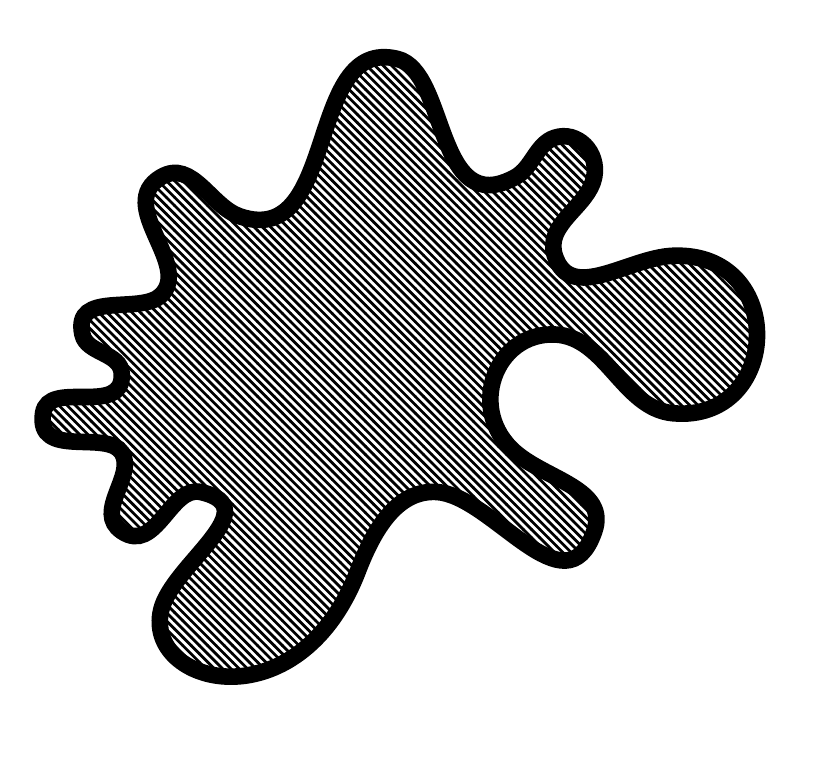
\begin{tikzpicture}[use Hobby shortcut,closed=true]
      \draw[pattern=custom north west lines,line width=6,hatchspread=3pt,hatchthickness=1pt,draw=black, rounded corners=0](-2.5,-0.5).. (-3.5,0).. (-2.5,0.5).. (-3,1).. (-2,1.5).. (-2,3).. (-1,2.5).. (1,4.5).. (2.5,3).. (3,3.5).. (3.5,3).. (3,2).. (4.5,2).. (4.5,0).. (3,1).. (2.5,-0.5).. (3.5,-1.5).. (1.5,-1).. (0.5,-2).. (-2,-2.5).. (-1.5,-1).. (-2.5,-1.5).. (-2.5,-0.5);
\end{tikzpicture}
}
}
%
%\newcommand{\figplug}[1]{\subfloat[Type~#1. \label{fig:Type#1}]{%
%  \begin{tikzpicture}
%  \node at (0,0){
%    \includegraphics[height=1cm]{plugs/#1-button}};
%  \end{tikzpicture}
%}}

\newcommand{\figplug}[1]{
 #1~\includegraphics[height=2cm,angle=-90,origin=c]{plugs/#1-button}
}

\newcommand{\comma}[2]{
\begin{tikzpicture}
\node at (0,0) {#1 \Huge{,}#2};
\end{tikzpicture}}


\newcommand{\cordG}[1]{%
  \raisebox{-2.6pt}{\includegraphics[width=4mm]{socket}}%
  \hspace{-1.3mm}%
  -#1-%
  \hspace{-1.3mm}\raisebox{-2.2pt}{\includegraphics[width=4mm]{plug}}}
%:nomenc:\cordG{\ell}: A cord of length $\ell$

\newcommand{\cord}[3]{
 \begin{tikzpicture}
 \node (flaga) at (0,0) {#1};
 \node[right=0.02cm of flaga] (sock) {\includegraphics[width=4mm]{socket}};
 \node[right=0.02cm of sock](lab) {$#2$};
  \draw ($(sock.east)+(-0.125,0)$) --  ($(lab.west)-(-0.05,0)$) {};
 \node[right=0.02cm of lab](plug){ \includegraphics[width=4mm]{plug}};
 \draw ($(lab.east)+(-0.075,0)$) --  ($(plug.west)+(0.125,0)$) {};
 \node[right=0.02cm of plug] {#3};
 \end{tikzpicture}
}

\newcommand{\homtemplate}[6]{
\begin{tikzpicture}
\node[block,draw=morphisms] (one) at (0,0) {$#1$};
\node[block, right=0.5cm of one, dashed, fill=yellow] (two) {};
\node[block, right=0.5cm of two,draw=morphisms] (three) {$#2$};
\draw[-, thick] (one.east) -- node[pos=0.5,above] {$#3$}(two.west) {};
\draw[-, thick] (two.east) -- node[pos=0.5,above] {$#4$}(three.west) {};
\draw[-, thick] ($(one.west)+(-0.5,0)$) -- node[pos=0.5,above] {$#5$}(one.west) {};
\draw[-, thick] (three.east) -- node[pos=0.5,above] {$#6$}($(three.east)+(0.5,0)$) {};
\end{tikzpicture}
}

%:nomenc:\TypeIrish}{c}{\TypeSwiss}: A cord with different types.

% \newcommand{\cord}[3]{{#1}\xrightarrow{#2}{#3}}
\newcommand{\TypeIrish}{\includegraphics[height=2mm]{flag-ireland}}
\newcommand{\TypeSwiss}{\includegraphics[height=2mm]{flag-swiss}}
\newcommand{\TypeFrench}{\includegraphics[height=2mm]{flag-france}}
\newcommand{\TypeItalian}{\includegraphics[height=2mm]{flag-italy}}
\newcommand{\TypeUSA}{\includegraphics[height=2mm]{flag-usa}}
\newcommand{\TypeChinese}{\includegraphics[height=2mm]{flag-china}}


\newcommand{\dashedbox}[1]{
%\scalebox{scale=0.8}{%
%dashed
\begin{tikzpicture}
\draw[#1, ultra thick, rounded corners=0] (-0.25,-0.25) rectangle (0.5,0.5){};
\end{tikzpicture}%
%}%
}

\newcommand{\dashedboxfilled}[2]{
%\scalebox{scale=0.8}{%
%dashed
\begin{tikzpicture}
\draw[#1, ultra thick, rounded corners=0] (-0.25,-0.25) rectangle node[pos=0.5, black]{#2} (0.5,0.5){};
\end{tikzpicture}%
%}%
}

\newcommand{\dashedboxinv}[2]{
%\scalebox{scale=0.8}{%
\begin{tikzpicture}
\draw[white, text=#2, ultra thick,dashed, rounded corners=0] (-0.25,-0.25) rectangle (0.5,0.5) node[pos=0.5, text=#2]{\textcolor{#2}{#1}};
\end{tikzpicture}%
%}%
}


\newcommand{\roundbox}[1]{
\begin{tikzpicture}
\draw[#1, ultra thick,dashed] (-0.25,-0.25) circle (0.35);
\end{tikzpicture}
}

\newcommand{\filledbox}[2]{
\begin{tikzpicture}
\draw[black, ultra thick,fill=#1] (-0.5,-0.275*#2) rectangle (1.5,0.55*#2){};
\end{tikzpicture}
}

\newcommand{\coloredbox}[1]{
\begin{tikzpicture}
\draw[#1, ultra thick,fill=#1] (-0.25,-0.25) rectangle (1, 0.5);
\end{tikzpicture}
}

\pgfdeclarelayer{background}
\pgfdeclarelayer{foreground}
\pgfsetlayers{background,main,foreground}

%
% #1 is color of main rope
% #2 is color of rope after knot
% #3 is x progress of the rope
% #4 is y progress of the rope
% #5 is position of first not (in [0,1])
% #6 is position of second not (in [0,1])
% #7 is label
\newcommand{\rope}[7]{
\begin{tikzpicture}[n/.style={circle,draw,minimum size=2mm,inner sep=0, fill=#1}, remember picture]
\ifthenelse{\lengthtest{#5 pt=0 pt} \AND \lengthtest{#6 pt=1 pt}}
{\draw[ultra thick, #1] (0,0) -- node[pos=#5, #1,n]{} node[pos=#6,n] {} node[pos=0.5, above, black]{#7} (#3,#4){};}
{\draw[ultra thick, #1] (#5*#3,#5*#4) -- node[pos=0, #1,n,overlay]{} node[pos=1, #1,n] {} node[pos=0.5, above, black]{#7} (#6*#3,#6*#4){};
\begin{pgfonlayer}{background}
\draw[ultra thick, #2] (0,0)--(#5*#3,#5*#4){};
\draw[ultra thick, #2] (#6*#3,#6*#4)--(#3,#4){};
\end{pgfonlayer}}
\end{tikzpicture}}


\newcommand{\northenb}{%
\mathbin{
\begin{tikzpicture}[n/.style={circle,draw,minimum size=0.8mm,inner sep=0, fill=black}]
\node[n] at (0,0.05) {};
\node[n] at (0.2,0.05) {};
\node at (0.1,0.1){};
\draw[thick](0,0.05)--(0.2,0.05){};
\end{tikzpicture}}}

\newcommand{\northena}{%
\mathbin{\begin{tikzpicture}[n/.style={circle,draw,minimum size=0.8mm,inner sep=0, fill=black}]
%\node[n] at (0,0.05) {};
\node[n] at (0.125,0.05) {};
\node at (0.1,0.1){};
\draw[thick](0,0.05)--(0.25,0.05){};
\end{tikzpicture}}}

% 1. color
% 2.3. position
%
\newcommand{\ropeknot}[6]{
\begin{tikzpicture}[n/.style={circle,draw,minimum size=2mm,inner sep=0, fill=#1}, m/.style={circle,draw,minimum size=1.5mm,inner sep=0, fill=none}, remember picture]
  \draw[#6,thick, fill=none] ($(#4,#5)-(0,0.25)$) -- node[pos=0, #6,m]{} node[pos=1, #6,m]{} ($(#4,#5)+(0,0.25)$){};
\draw[ultra thick, #1] (0,0) -- node[pos=0, #1,n]{} node[pos=1, #1,n]{} (#2,#3){};
\end{tikzpicture}}


\usepackage{forest}

\newcommand{\dirtree}[1]{%
    \begin{forest}
      for tree={
        font=\ttfamily,
        grow'=0,
        child anchor=west,
        parent anchor=south,
        anchor=west,
        calign=first,
        edge path={
          \noexpand\path [draw, \forestoption{edge}]
          (!u.south west) +(4.5pt,0) |- node[fill,inner sep=1.25pt] {} (.child anchor)\forestoption{edge label};
        },
        before typesetting nodes={
          if n=1
            {insert before={[,phantom]}}
            {}
        },
        fit=band,
        before computing xy={l=15pt},
      }
    #1
    \end{forest}
}

%
%
%\tikzset{
%  font={\fontsize{10pt}{12}\selectfont}}
\definecolor{cblue}{rgb}{0.3,0.3,1.0}
\definecolor{cred}{rgb}{1.0,0.1,0.1}

\definecolor{cwhite}{rgb}{0.95,0.95,0.97}
\definecolor{funbox}{rgb}{0.92,1,0.9}
\definecolor{resbox}{rgb}{1,0.74,0.75}
\definecolor{impbox}{rgb}{1,0.92,0.85}

\newcommand{\legob}[1]{%
\adjustbox{scale=0.4}{\includesag{intro-lego-#1}}%
}

\usetikzlibrary{shadows.blur}
\usetikzlibrary{shapes.symbols}

\newcommand{\shadowbox}[1]{
\begin{tikzpicture}
\node[draw=gray,shade,
      top color=white,
      bottom color=white,
      rounded corners=6pt,
      blur shadow={shadow blur steps=6}
    ] {#1};
\end{tikzpicture}}

\definecolor{red1}{rgb}{0.30,0,0}
\definecolor{red2}{rgb}{0.60,0,0}
\definecolor{red3}{rgb}{0.90,0,0}
\definecolor{my-cyan}{cmyk}{1,0,0,0}
\definecolor{my-magenta}{cmyk}{0,1,0,0}
\definecolor{my-yellow}{cmyk}{0,0,1,0}
%


\newcommand{\funbox}[3]{
\begin{tikzpicture}
\node[draw=funbox,
      fill=funbox,
      minimum height =2cm,
minimum width =2cm,
      rounded corners=6pt] at (#1,#2) {#3};
\end{tikzpicture}}

\newcommand{\resbox}[3]{
\begin{tikzpicture}
\node[draw=resbox,
      fill=resbox,
      minimum height =2cm,
minimum width =2cm,
      rounded corners=6pt] at (#1,#2) {#3};
\end{tikzpicture}}

\newcommand{\impbox}[3]{
\begin{tikzpicture}
\node[draw=impbox,
      fill=impbox,
      minimum height =2cm,
minimum width =2cm,
      rounded corners=6pt] at (#1,#2) {#3};
\end{tikzpicture}}

\newcommand{\boxset}[1]{
\begin{tikzpicture}
\node[draw=setcolor,
      fill=setcolor,
      rounded corners] at (0,0) {#1};
\end{tikzpicture}}

\tikzcdset{
    setcd/.style={
        every matrix/.append style={
            draw=setcolorbord,
            fill=setcolor,
            rounded corners,
            inner sep=1pt,
            #1
        },
    },
}

\tikzcdset{
    posetcd/.style={
        every matrix/.append style={
            draw=posetcolorbord,
            fill=posetcolor,
            rounded corners,
            inner sep=1pt,
            #1
        },
    },
}

\tikzcdset{
    catcd/.style={
        every matrix/.append style={
            draw=catcolor,
            fill=catcolor,
            rounded corners,
            inner sep=4pt,
            #1
        },
    },
}

\tikzcdset{
    graphcd/.style={
        every matrix/.append style={
            draw=graphcolorbord,
            fill=graphcolor,
            rounded corners,
            inner sep=4pt,
            #1
        },
    },
}

% label bottom right
\newcommand{\labelobleft}[2]{
    \node[left=0mm of #1.south west, anchor=south east] {#2};
}
% label above
\newcommand{\labelobtop}[2]{
    \node[above left=0mm of #1.north west, anchor=south west] {#2};
}

\newcommand{\arrowbgcolor}{white}
